% 2015_shandong_science_q17: triangular frustum DEF-ABC with interior lines (same drawing as liberal)
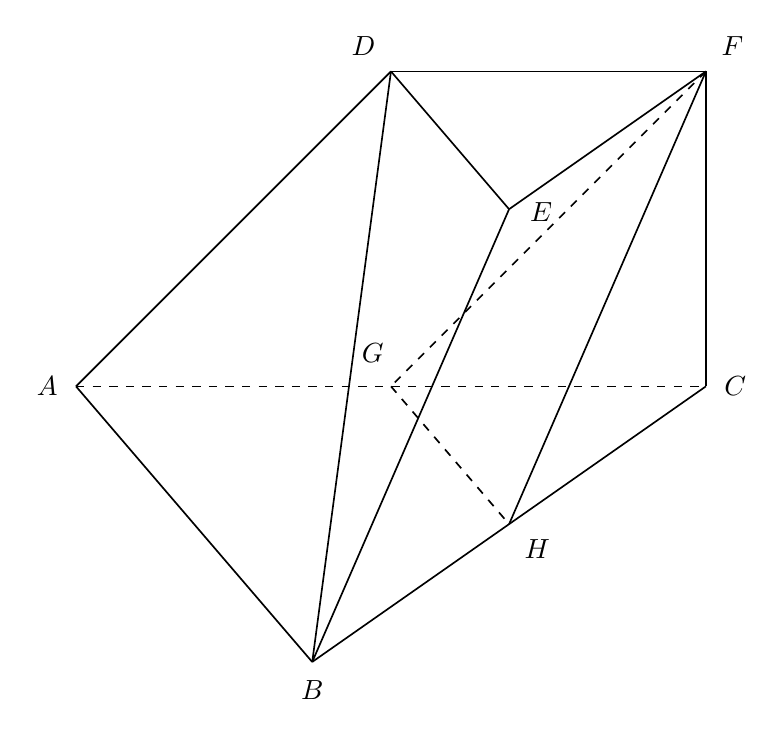
\begin{tikzpicture}[line width=0.6pt, font=\normalsize]
\coordinate (A) at (-4,0);
\coordinate (C) at (4,0);
\coordinate (B) at (-1,-3.5);
\coordinate (D) at (0,4);
\coordinate (F) at (4.0000000000,4.0000000000);
\coordinate (E) at (1.5000000000,2.2500000000);
\coordinate (G) at (0.0000000000,0.0000000000);
\coordinate (H) at (1.5000000000,-1.7500000000);
% outline / solid edges
\draw (A)--(B);
\draw (A)--(D);
\draw (B)--(D);
\draw (B)--(E);
\draw (B)--(C);
\draw (D)--(F);
\draw (D)--(E);
\draw (E)--(F);
\draw (F)--(C);
\draw (F)--(H);
% hidden edges
\draw[dashed] (A)--(C);
\draw[dashed] (F)--(G);
\draw[dashed] (G)--(H);
% labels with clearance from strokes
\node[left=3pt] at (A) {$A$};
\node[below=3pt] at (B) {$B$};
\node[right=3pt] at (C) {$C$};
\node[above left=2pt] at (D) {$D$};
\node[above right=2pt] at (F) {$F$};
\node[right=3pt,xshift=1.0pt,yshift=-1.0pt] at (E) {$E$};
\node[above left=4pt,xshift=5pt,yshift=1pt] at (G) {$G$};
\node[below right=2pt] at (H) {$H$};
\end{tikzpicture}
